\documentclass[12pt]{beamer}
\usetheme{Darmstadt}
\usepackage{graphicx}
\usepackage[ngerman]{babel}
\usepackage[T1]{fontenc}
\usepackage[utf8]{inputenc}
\usepackage{tikz}
\usepackage[shadow,colorinlistoftodos]{todonotes}
\setbeamertemplate{footline}[frame number]

\newcommand{\cc}[1]{\includegraphics[height=4mm]{img/#1.png}}
\usepackage{ifthen}
\newcommand{\license}[2][]{\\#2\ifthenelse{\equal{#1}{}}{}{\\\scriptsize\url{#1}}}
\usepackage{textcomp}

%\setbeamercovered{transparent}

\pgfdeclareimage[height=.6cm]{c3d2logo}{./img/c3d2.pdf} 


\pgfdeclarelayer{foreground}
\pgfsetlayers{main,foreground}
\logo{\pgfputat{\pgfxy(-1,0)}{\pgfbox[center,base]{\pgfuseimage{c3d2logo}}}}


\title{Medienkompetenz}
\author{\small Stephan Thamm, Nerd Norbert \& Benjamin Partzsch \\\large Chaos Computer Club Dresden}
\date{22.05.2018}

\begin{document}
\maketitle

\section*{Einleitung}
\subsection*{}

%%% -> thammi -> %%%

\begin{frame}
  \frametitle{Hacker}
  \begin{figure}
    \only<2>{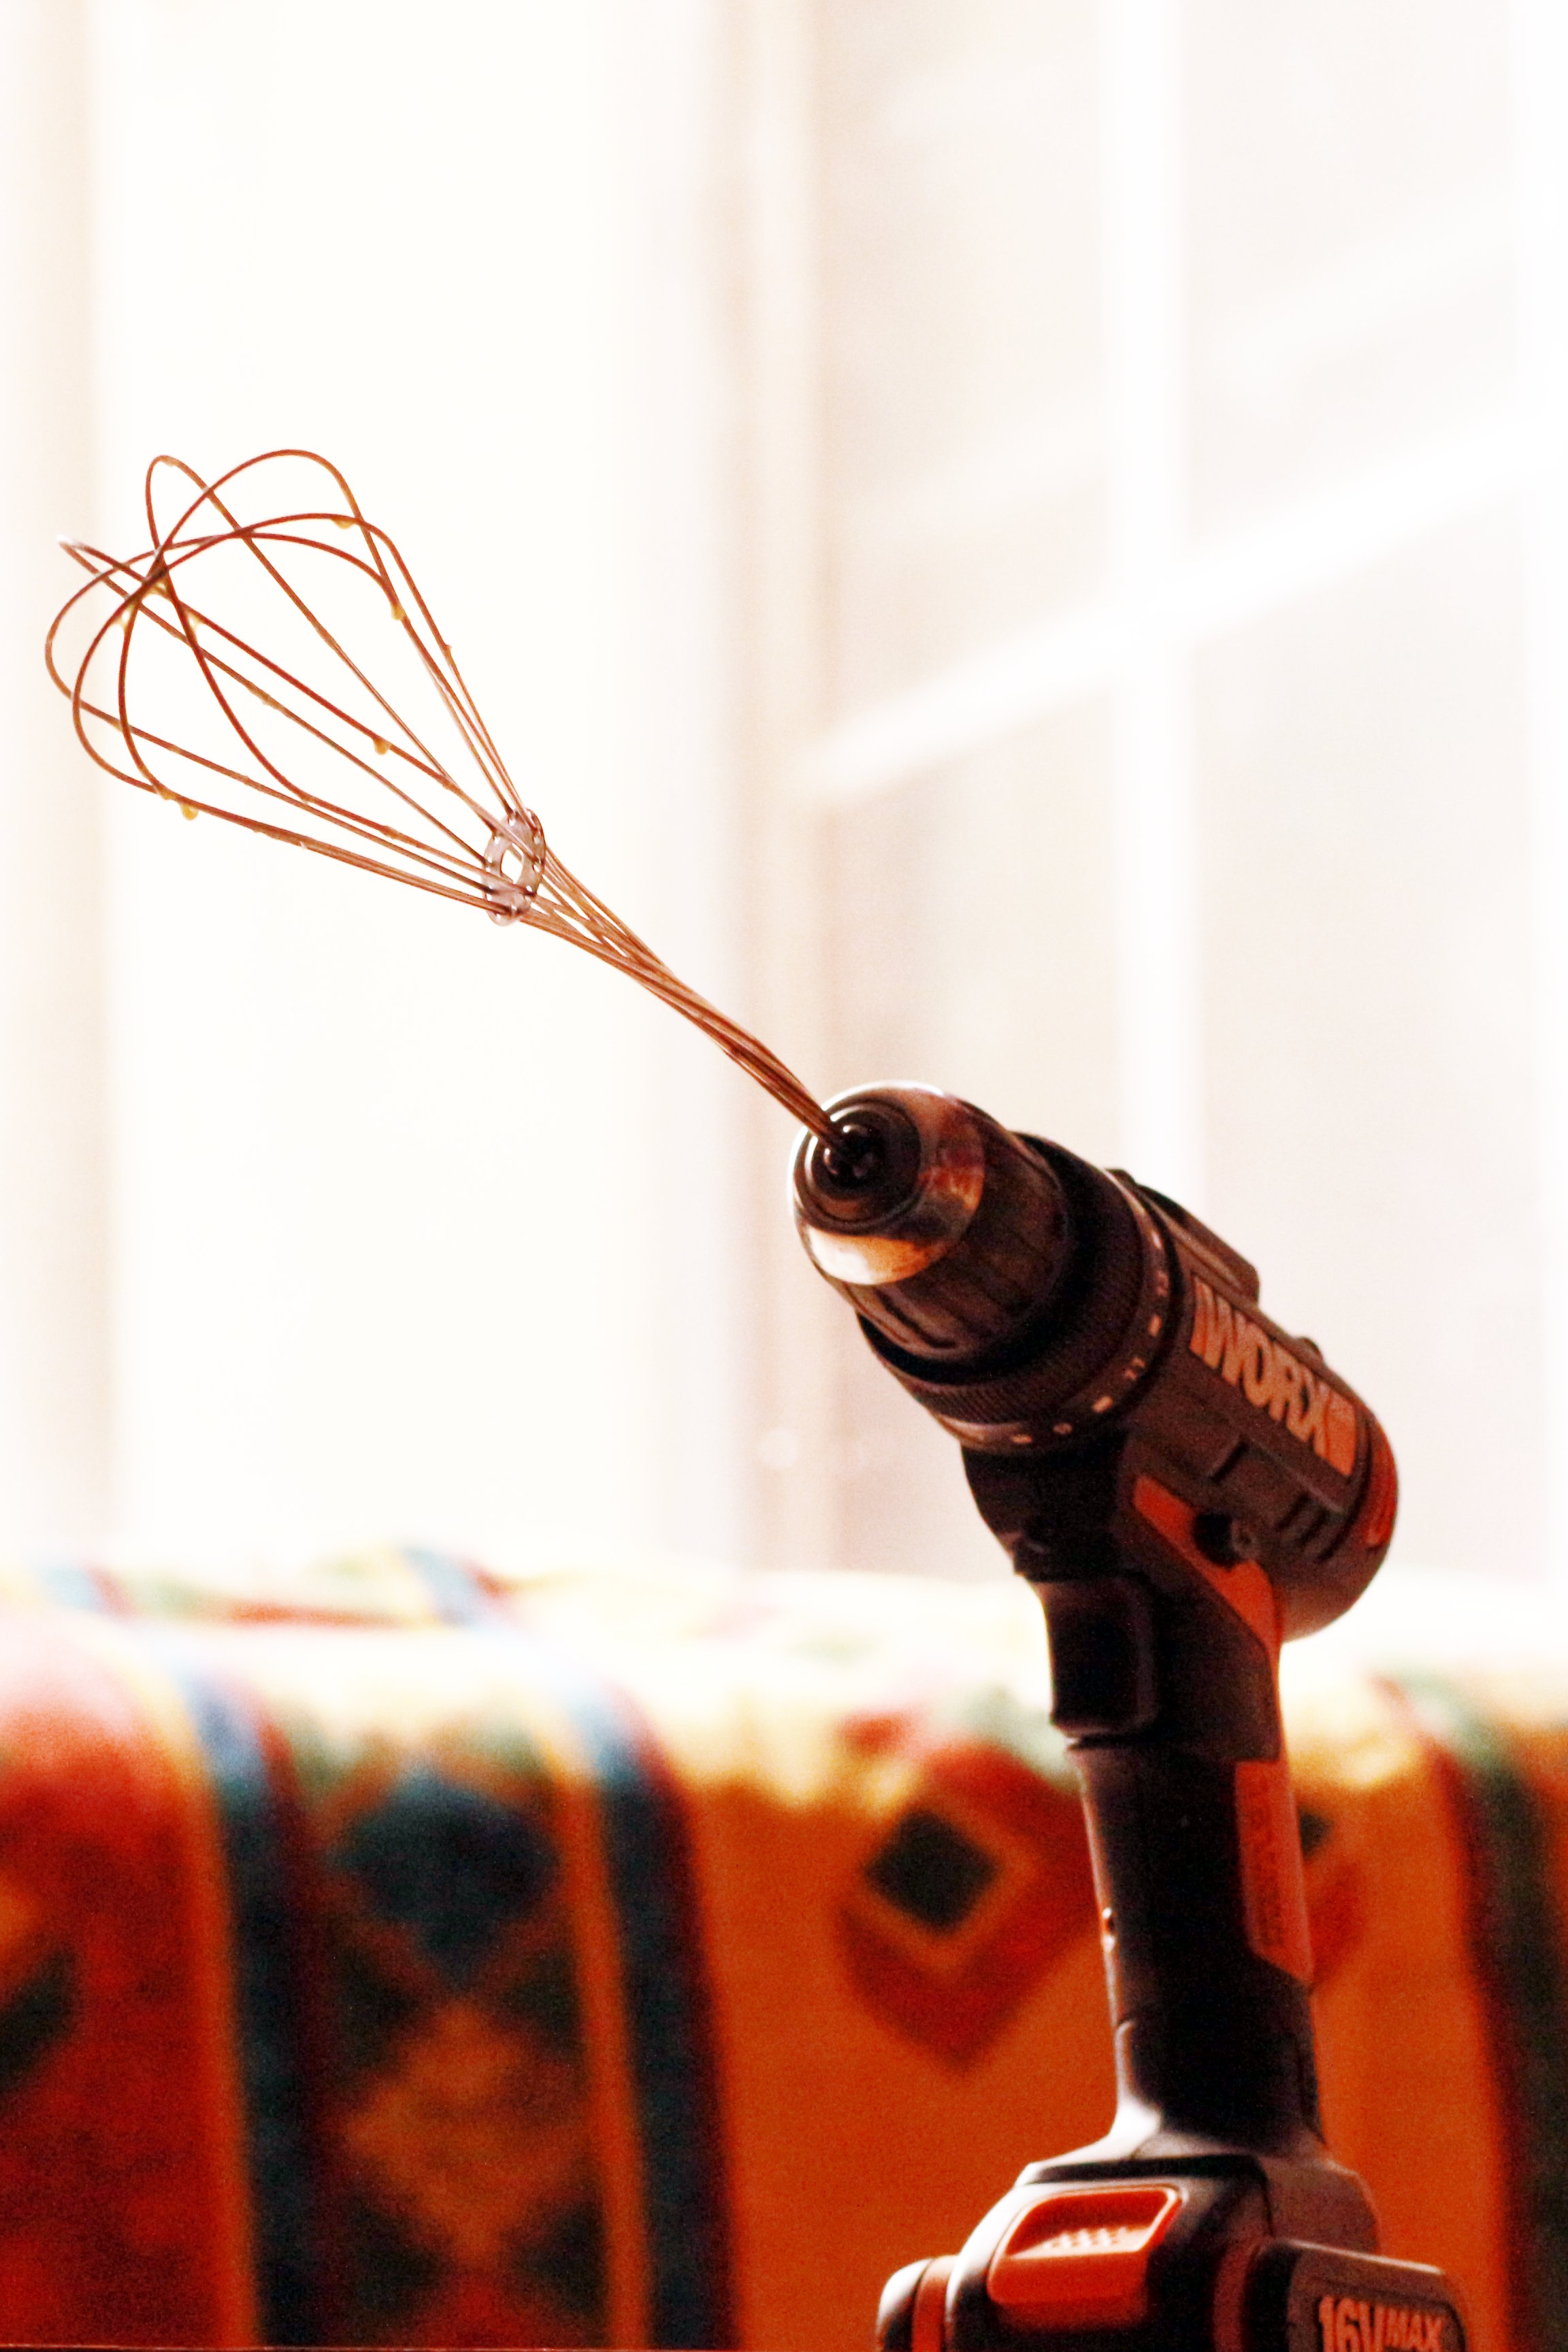
\includegraphics[height=0.7\textheight]{img/schneeschrauber.jpg}}
    \only<3>{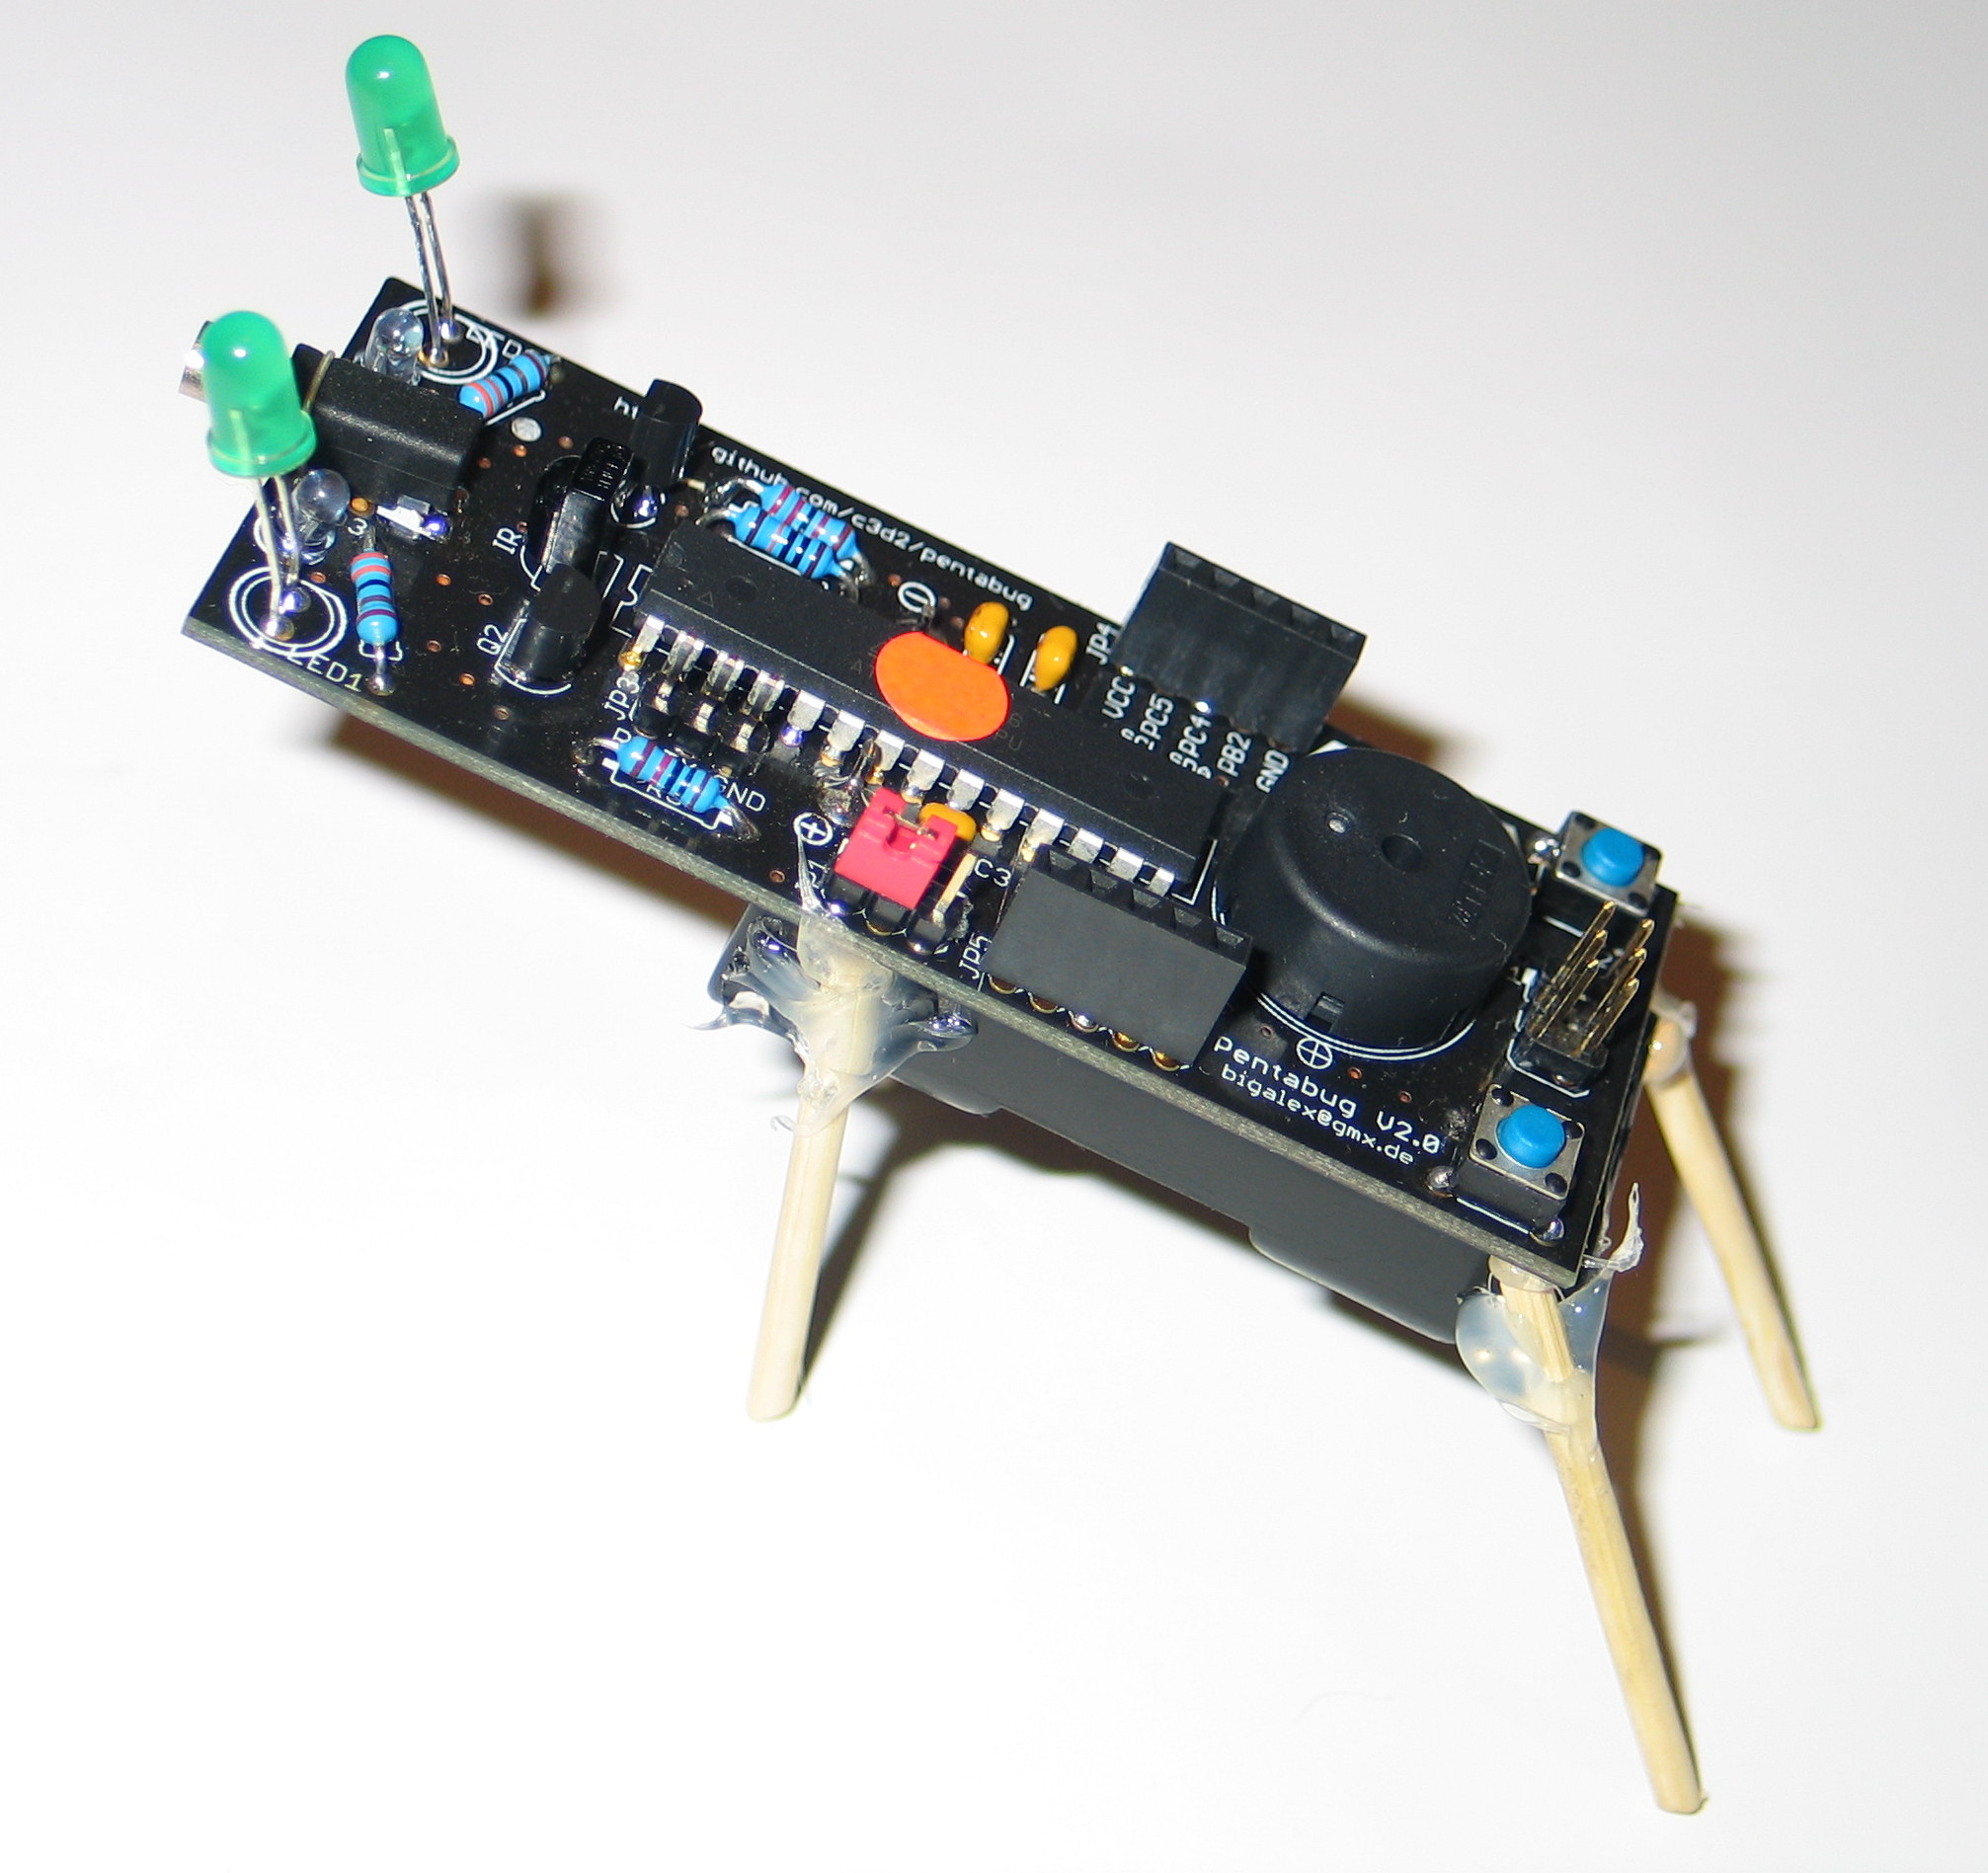
\includegraphics[height=0.7\textheight]{img/pentabug.jpg}}
  \end{figure}
\end{frame}

\begin{frame}
	\frametitle{Chaos Computer Club}
	\begin{center}
		
\includegraphics[height=0.2\textheight]{img/chaosknoten.png}
	\end{center}	
	\begin{itemize}
		\item Verein wurde 1981 gegründet (\url{https://ccc.de})          
		\item Aktuell mehr als 6000 Mitglieder
		\item Betreibt u.a. Öffentlichkeitsarbeit und Politikberatung      
		\item Lokale Erfahrungsaustauschkreise (Erfas) und Chaostreffs
	\end{itemize}
\end{frame}

\begin{frame}
	\frametitle{Chaos Computer Club Dresden}
	\begin{center}
		
\includegraphics[height=0.1\textheight]{img/c3d2_logo.png}
	\end{center}
	\begin{itemize}
		\item Chaos Computer Club Dresden (\url{https://c3d2.de})          
		\item Datenspuren (\url{https://datenspuren.de})
		\item Radio und Podcasts (\url{https://c3d2.de/radio.html})
		\item Chaos macht Schule (\url{https://c3d2.de/schule.html})
	\end{itemize}
\end{frame}

\begin{frame}
	\frametitle{Was bieten wir?}
	\begin{itemize}
		\item<2-> keine Pädagogen
		\item<3-> keine Rechtsanwälte
		\item<4-> keine technische Lösungen für soziale Probleme
		\item<5-> Hintergrundwissen und Denkanstöße
	\end{itemize}
\end{frame}

\begin{frame}{Themen}
\tableofcontents
\end{frame}

\section{Soziale Medien}
\subsection{}

\begin{frame}
  \frametitle{Soziale Medien}
  \begin{center}
    \only<2>{\huge Soziale Netzwerke}
    \only<3>{\huge Nachrichtendienste}
  \end{center}
\end{frame}

\begin{frame}
    \frametitle{Kostenlos?}
    \uncover{
        \begin{figure}
            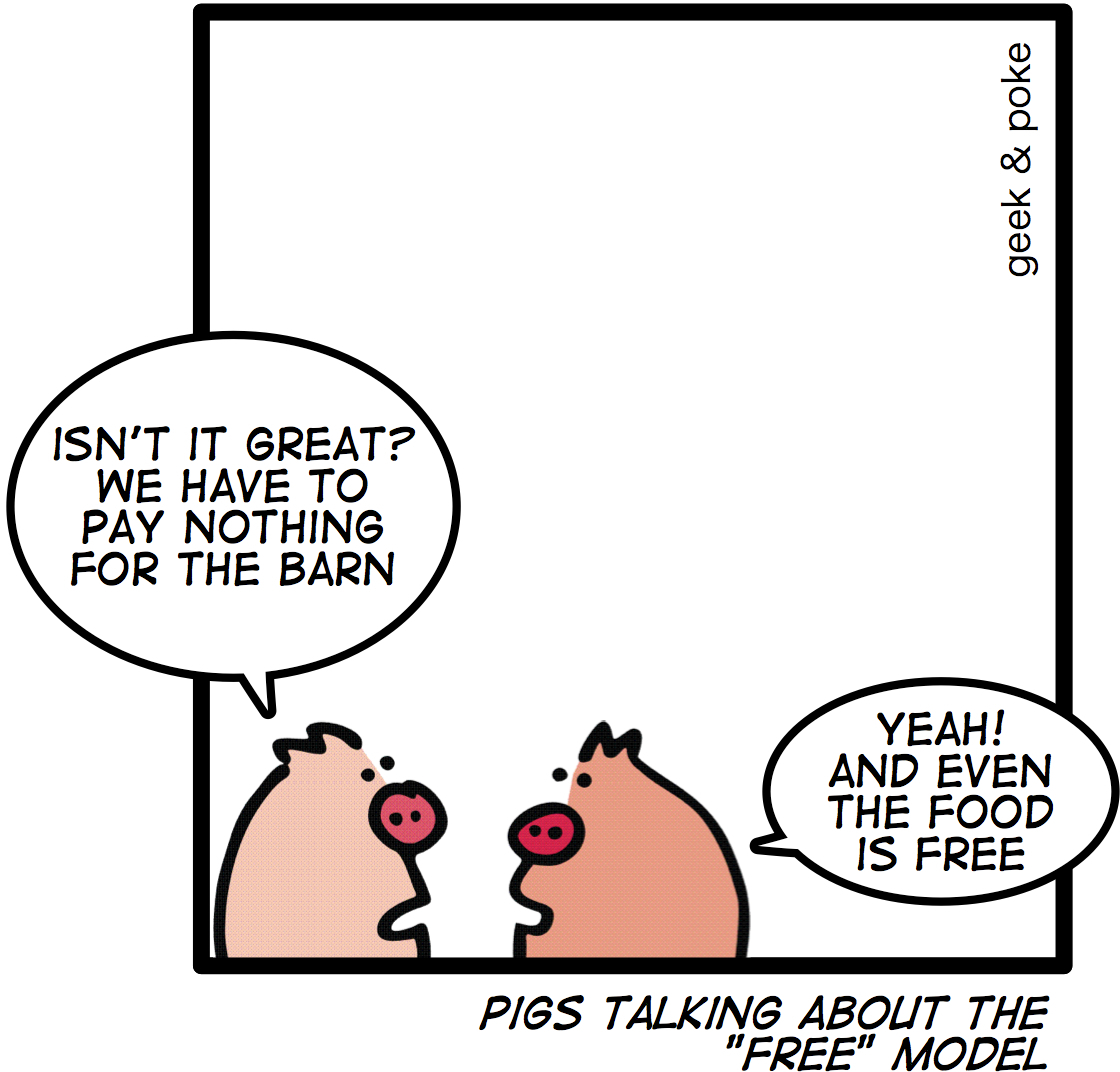
\includegraphics[height=0.6\textheight]{img/business_pigs.jpg}
            \license[http://geekandpoke.typepad.com/geekandpoke/2010/12/the-free-model.html]{\cc{by-sa}}
    \end{figure}}
\end{frame}

\begin{frame}
  \frametitle{Wert von Daten}
  \begin{figure}
    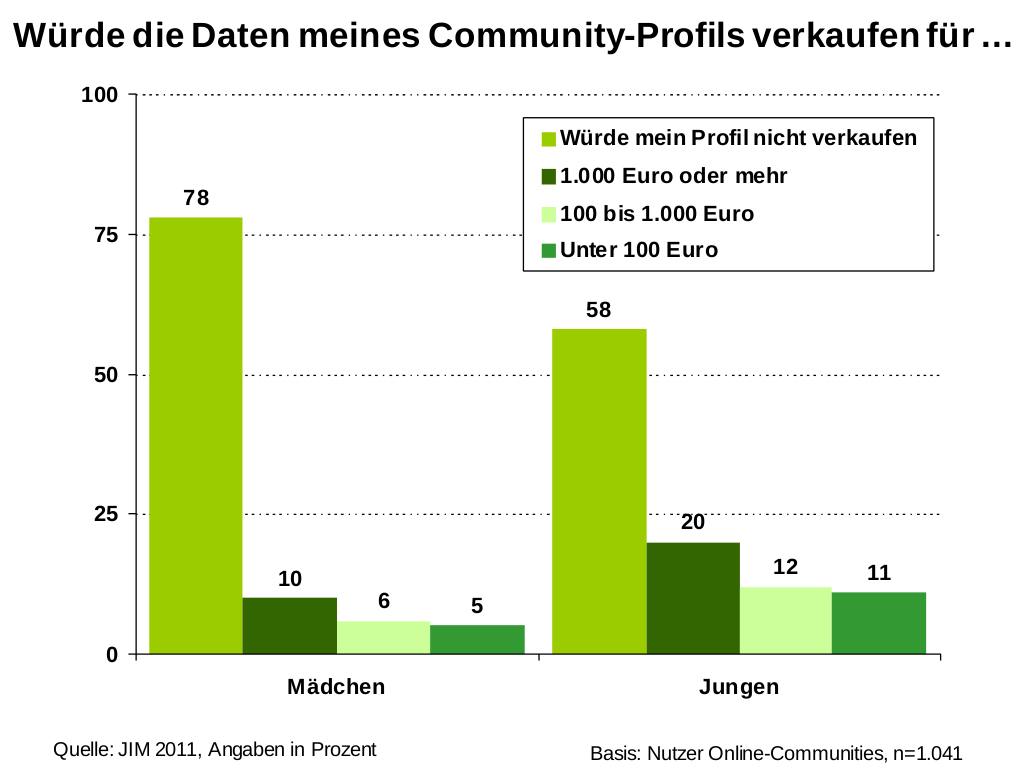
\includegraphics[height=0.7\textheight]{img/jim_verkaufen.png}
  \end{figure}
\end{frame}

\begin{frame}
	\frametitle{Personenbezogene Daten}
	\begin{itemize}
		\item<2-> Recht auf Vergessen?
		\item<3-> Das Internet vergisst nicht!
		\item<4-> Bundesdatenschutzgesetz und DSGVO
		\item<5-> Datenschutzerklärung
		\item<6-> Datenschutzeinstellungen und Zugriffsrechte
	\end{itemize}
\end{frame}

\begin{frame}
  \frametitle{Lock in effect}
  \begin{center}
    ``Tie all of our products together, so we further lock customers into our ecosystem'' (Steve Jobs)
  \end{center}
\end{frame}

%%% -> norbert -> %%%

\section{Sichere Mediennutzung}
\subsection{}

\begin{frame}
	\frametitle{Smartphone}
	\begin{itemize}
		\item<1-> Umfrage: Wessen Kinder nutzen ein Smartphone?
		\item<2-> Wozu?
	\end{itemize}
\end{frame}

\begin{frame}
	\frametitle{Smartphone}
	\begin{itemize}
		\item<1-> Betriebssysteme: Hersteller vs. Community
		\item<2-> App-Stores: Kommerziell vs. Open Source (F-Droid)
		\item<3-> Initiative vs. Delegation
		\item<4-> Notfall: Ortung, IMEI, Notruf Nummer
	\end{itemize}
\end{frame}

\begin{frame}
	\frametitle{Internet}
	\begin{itemize}
		\item<1-> Router: Innere Zugangskontrolle
		\item<2-> Firewall: Äußere Zugangskontrolle
		\item<3-> Proxy: Filterung
		\item<4-> Suchmaschine: Auwahl
		\item<5-> Was will ich erreichen?
	\end{itemize}
\end{frame}

\begin{frame}
	\frametitle{Vertrauen}
	\begin{itemize}
		\item<1-> Smartphone Hersteller
		\item<2-> Netzbetreiber
		\item<3-> Programm-Entwickler
		\item<4-> Webseitenbetreiber
		\item<5-> Eigene Kinder
	\end{itemize}
\end{frame}

%%% -> benhamin -> %%%

\section{Kreative Mediennutzung}
\subsection{}


\begin{frame}
	\frametitle{Benutzung von Software}
	\begin{itemize}
		\item<1-> Lernen
		\item<2-> Spielen / kreatives Gestalten
	\end{itemize}
	
	\begin{itemize}
		\item<3-> Ziele?
		\item<4-> auf welchem Gerät?
		\item<5-> Online oder installierbares Programm?
		\item<6-> OpenSource!
	\end{itemize}
	
	\begin{itemize}
		\item<7-> Erfahrungsaustausch unter Eltern
		\item<8-> Fach- und Klassenlehrer Fragen
	\end{itemize}
\end{frame}

\begin{frame}
	\frametitle{Software zum Lernen}
	\uncover<1->{Unterscheidung}
	\begin{itemize}
		\item<2-> Lernprogramme (Lernkartei Software, Vokabeltrainer)
	    \item<3-> Lernspiele (Spiel aber der Erwerb von Wissen liegt im Fordergrund)
	\end{itemize}
	\uncover<4->{Beispiele}
	\begin{itemize}
		\item<5-> App: Anki - im F-Droid App-Store
	    \item<6-> Online: schlaukopf.de - werbefinanziert!
	\end{itemize}
	\uncover<7->{Für die Weiterführende Schule:}
	\begin{itemize}
		\item<8-> https://www.geogebra.org/ - Mathemathik
		\item<9-> http://stellarium.org/ - Astronomie
		\item<10-> https://edu.kde.org/kalzium/ - Chemie
	\end{itemize}
\end{frame}

\begin{frame}
	\frametitle{Software zum Spielen / kreativen Gestalten}
	Spielen - Minetest
	\begin{center}
		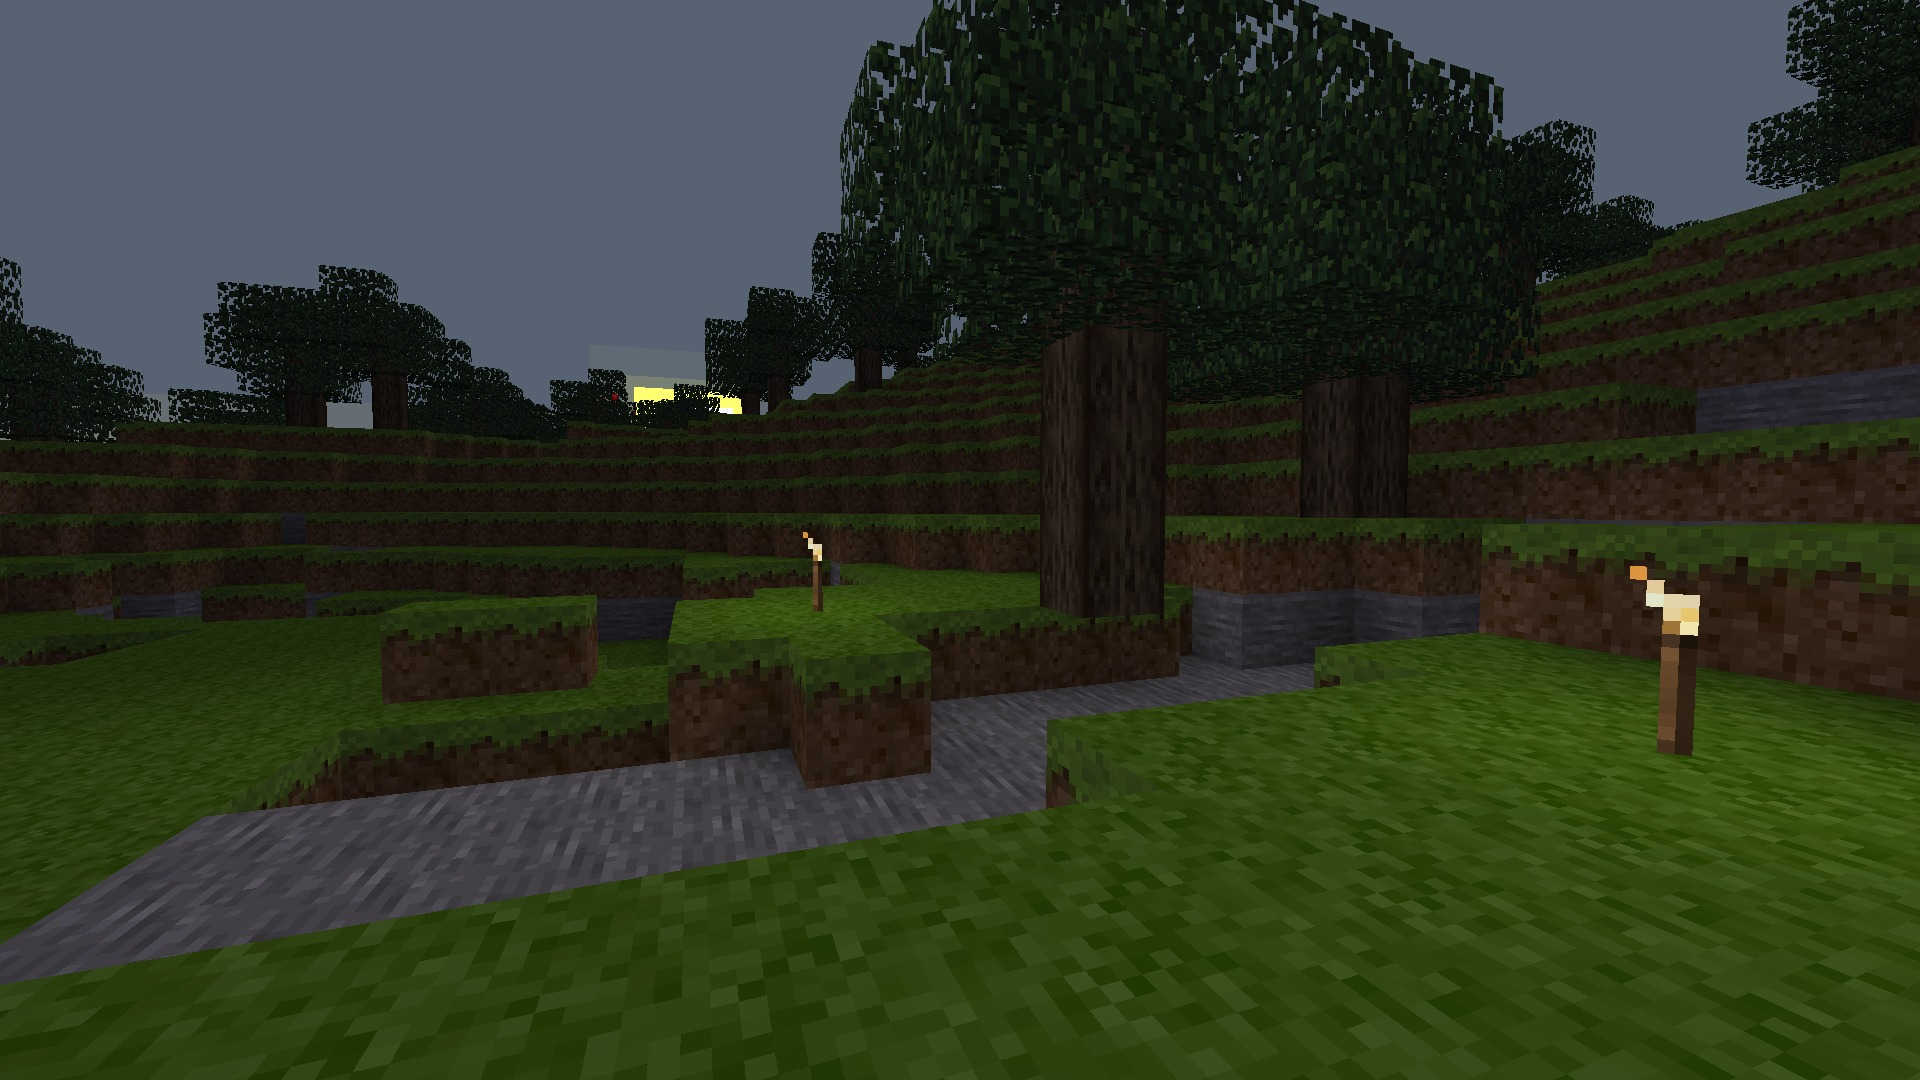
\includegraphics[height=0.6\textheight]{img/minetest.jpg}
	\end{center}
	https://wiki.minetest.net/Minetest\_in\_der\_Schule
\end{frame}

\begin{frame}
	\frametitle{Software zum Spielen / kreativen Gestalten}
	Konstruieren - LeoCAD 
	\begin{center}
		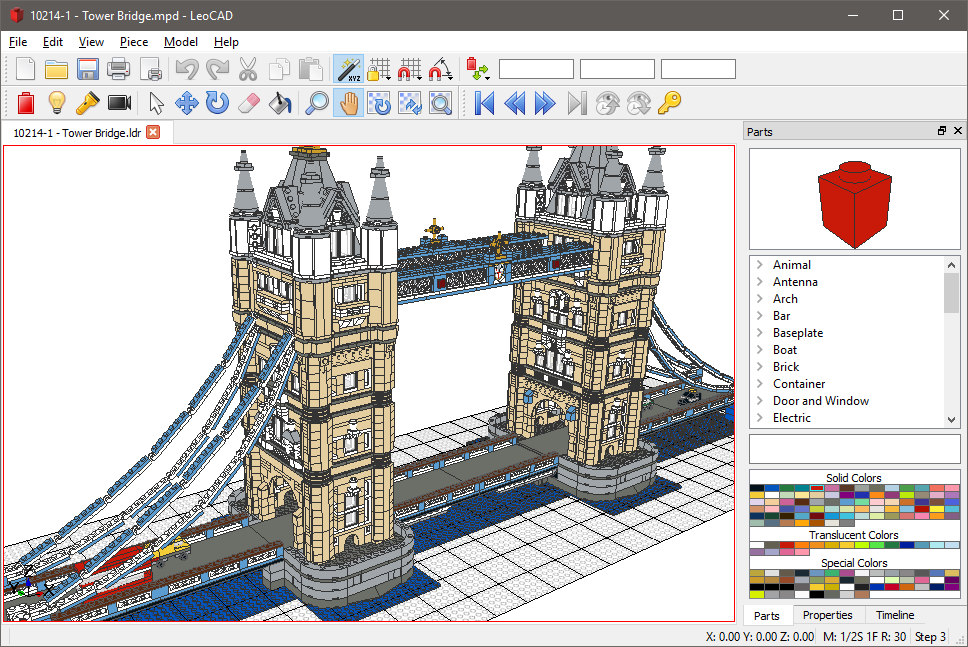
\includegraphics[height=0.6\textheight]{img/towerbridge.png}
	\end{center}
	https://www.leocad.org/
\end{frame}

\begin{frame}
	\frametitle{Software zum Spielen / kreativen Gestalten}
	Programmieren - Scratch
	\begin{center}
		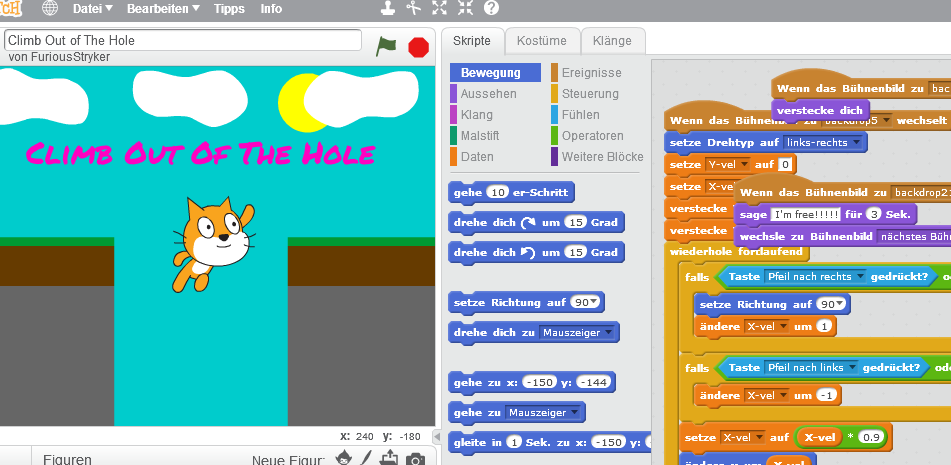
\includegraphics[height=0.6\textheight]{img/scratch.png}
	\end{center}
	https://scratch.mit.edu/
\end{frame}

%%% -> Ende -> %%%

\begin{frame}
	\frametitle{Ende}
	\begin{center}
		\textbf{Kontakt: schule@c3d2.de} \\
		\textbf{Fragen?} 
	\end{center}
	\begin{itemize}
		\item https://c3d2.de
		\item https://c3d2.de/schule.html
	\end{itemize}
\end{frame}

\end{document}
